% Opcje klasy 'iithesis' opisane sa w komentarzach w pliku klasy. Za ich pomoca
% ustawia sie przede wszystkim jezyk i rodzaj (lic/inz/mgr) pracy, oraz czy na
% drugiej stronie pracy ma byc skladany wzor oswiadczenia o autorskim wykonaniu.
\documentclass[declaration,shortabstract,inz]{iithesis}

\usepackage[utf8]{inputenc}
\usepackage{graphicx}
\usepackage{caption}

\graphicspath{{img/}}

%%%%% DANE DO STRONY TYTUŁOWEJ
% Niezaleznie od jezyka pracy wybranego w opcjach klasy, tytul i streszczenie
% pracy nalezy podac zarowno w jezyku polskim, jak i angielskim.
% Pamietaj o madrym (zgodnym z logicznym rozbiorem zdania oraz estetyka) recznym
% zlamaniu wierszy w temacie pracy, zwlaszcza tego w jezyku pracy. Uzyj do tego
% polecenia \fmlinebreak.
\polishtitle    {Badanie gier kooperacyjnych z niepełną\fmlinebreak informacją na przykładzie gry Hanabi}
\englishtitle   {A study on cooperative games with incomplete\fmlinebreak information based on the game of Hanabi}
\polishabstract {\ldots}
\englishabstract{\ldots}
% w pracach wielu autorow nazwiska mozna oddzielic poleceniem \and
\author         {Wojciech Jarząbek \and
				Jacek Leja}
% w przypadku kilku promotorow, lub koniecznosci podania ich afiliacji, linie
% w ponizszym poleceniu mozna zlamac poleceniem \fmlinebreak
\advisor        {dr Paweł Rychlikowski}
%\date          {}                     % Data zlozenia pracy
% Dane do oswiadczenia o autorskim wykonaniu
%\transcriptnum {}                     % Numer indeksu
%\advisorgen    {dr. Pawła Rychlikowskiego} % Nazwisko promotora w dopelniaczu
%%%%%

%%%%% WLASNE DODATKOWE PAKIETY
%
%\usepackage{graphicx,listings,amsmath,amssymb,amsthm,amsfonts,tikz}
%
%%%%% WŁASNE DEFINICJE I POLECENIA
%
%\theoremstyle{definition} \newtheorem{definition}{Definition}[chapter]
%\theoremstyle{remark} \newtheorem{remark}[definition]{Observation}
%\theoremstyle{plain} \newtheorem{theorem}[definition]{Theorem}
%\theoremstyle{plain} \newtheorem{lemma}[definition]{Lemma}
%\renewcommand \qedsymbol {\ensuremath{\square}}
% ...
%%%%%

\let\cleardoublepage=\clearpage

\begin{document}

\chapter{Wprowadzenie}

\section{Czym jest Hanabi?}

Gry planszowe to forma rozrywki, która towarzyszy człowiekowi od~tysięcy lat. Były one popularne już za~czasów antycznych, czego dowodzi chociażby malowidło z~3300~r.~p.n.e, pochodzące z~grobowca Merknery, na~którym ukazano rozgrywkę Seneta. Przykładem może być także Królewska~Gra~z~Ur, której egzemplarze odnaleziono w~trakcie badań nad~starożytną Mezopotamią. Choć gry te zostały w~dzisiejszych czasach w~znacznej mierze zapomniane, nie~sposób nie~wspomnieć o~innych z~podobnego okresu, takich~jak~warcaby czy~Go, a~także o~nieco młodszych szachach, które wciąż cieszą~się ogromną i~niesłabnącą popularnością.

Każdą z~tych gier łączy aspekt rywalizacji: pod~koniec rozgrywki jednoznacznie wyszczególnia~się jednego lub~więcej graczy, których określamy mianem zwycięzców, zaś~reszta -~przegrywa. Inne podejście prezentują gry kooperacyjne, gdzie zadaniem nie~jest pokonanie innych uczestników zabawy, a~osiągnięcie wspólnego celu, który gwarantuje wygraną. Można powiedzieć, że~przeciwnikiem graczy jest w~tym przypadku sama gra, która swoją konstrukcją skłania do~współpracy. Pierwsze gry tego typu powstały dopiero w~drugiej połowie XX~wieku i~początkowo miały wyłacznie charakter edukacyjny. Wraz z~popularyzacją tzw. ``planszówek'' gry kooperacyjne w~znacznym stopniu zyskały na~popularności, a~ich forma wyewoluowała w~kierunku zabawy kładącej nacisk na~aspekty towarzyskie, które ograniczają lub~wręcz odrzucają współzawodnictwo. Przykładami takiego podejścia mogą~być Pandemic, Martwa Zima, a~także Hanabi.

Hanabi (jap. fajerwerki) to~w~pełni kooperacyjna gra planszowa, która w~2013 roku wygrała prestiżową nagrodę Spiel~des~Jahres. Gracze wcielają~się w~niej w pracowników fabryki fajerwerków, w~której omyłkowo zostały pomieszane ze~sobą różne rodzaje prochu. Celem jest złożenie w~odpowiedniej kolejności możliwie jak~największej ilości sztucznych ogni, które gracze otrzymują poprzez dobieranie kart z~potasowanej talii. Uczestnicy rozgrywki widzą karty, które są~w~posiadaniu innych graczy, lecz~nie~mogą przypatrywać~się~tym, którymi sami dysponują. Dodatkowo, komunikacja odnosząca~się do~treści kart podlega restrykcyjnym zasadom i~jest w~znacznym stopniu ograniczona, co~czyni rozgrywkę nietrywialną. Jakie strategie należy zatem zastosować, by~wygrać? Jak można przełożyć je~na~świat algorytmów?

\section{Hanabi a sztuczna inteligencja}

W~teorii gier istnieje pojęcie perfekcyjnego zagrania, czyli pojedynczego ruchu zależnego od~aktualnego etapu gry, prowadzącego do~stanu rozgrywki maksymalizującego oczekiwany wynik, niezależnie od~ruchów, które mogą w~odpowiedzi wykonać inni gracze. Perfekcyjne zagrania są~podstawą optymalnego planu działania, minimalizującego możliwe straty ponoszone w~trakcie rozgrywania danej partii. Niestety, tak~silna strategia -~w~przypadku złożonych gier -~jest nieprawdopodobnie trudna do~uzyskania ze~względu na~ogromną rozpiętość drzewa możliwych do~uzyskania stanów rozgrywki. W~praktyce używa~się algorytmów: heurystycznych, regułowych, opartych na~technikach uczących, nadużywających zasad gry lub~siłowych. Przykładowo, słynny komputer Deep Blue, który w~maju 1997 roku pokonał ówczesnego mistrza świata w~szachach, Garrego Kasparova, nie~posiadał optymalnej strategii. Używał on~w~zamian metody siłowej, wspomaganej algorytmem przeszukującym alfa-beta, rozpatrując wszystkie możliwe zagrania i~wybierając~te, które dawały mu~największą przewagę lokalną. Takie podejście było możliwe z~racji na ogromną moc superkomputera, który potrafił rozpatrywać 200~milionów ruchów na~sekundę.

Stworzenie sztucznej inteligencji do~Hanabi to~zadanie, które wymaga pokonania trudności niespotykanych w~innych grach. Jest to~następstwo kilku czynników: niepełnej informacji, losowości dobieranych kart, a~także ograniczonych zasobów, m.in. w~postaci podpowiedzi dla~innych graczy. Agenci muszą sobie ufać, gdyż gracz, który nie~chce współpracować, może w~kilku ruchach doprowadzić do~przegranej całej grupy. Ważne jest, by~nie~marnować zasobów, a~zatem sztuczna inteligencja musi być odpowiednio skoordynowana z~innymi graczami. Ponadto, znikoma ilość kart w~talii nie~pozwala na~zbyt długą rozgrywkę -~oznacza to~zatem, że~aby zdążyć z~wygraną, agenci muszą posiadać protokół komunikacji, który dopuszcza przekazywanie w~obrębie zasad gry dodatkowych, implicytnych informacji, rozumianych przez pozostałych jej~uczestników.

Niniejsza praca ma~na~celu zbadanie Hanabi jako gry kooperacyjnej z~niepełną informacją. Będziemy analizować techniki tworzenia agentów sztucznej inteligencji grających w~Hanabi, którzy wykonują możliwie najbardziej efektywne i~zrozumiałe dla ludzi ruchy na~tyle szybko, by~umożliwić komfortową rozgrywkę z~człowiekiem na~zwykłych komputerach.


\chapter{Reguły gry}

\renewcommand{\thefigure}{1}
\begin{figure}[ht!]
	\centering
	\captionsetup{format=hang}
	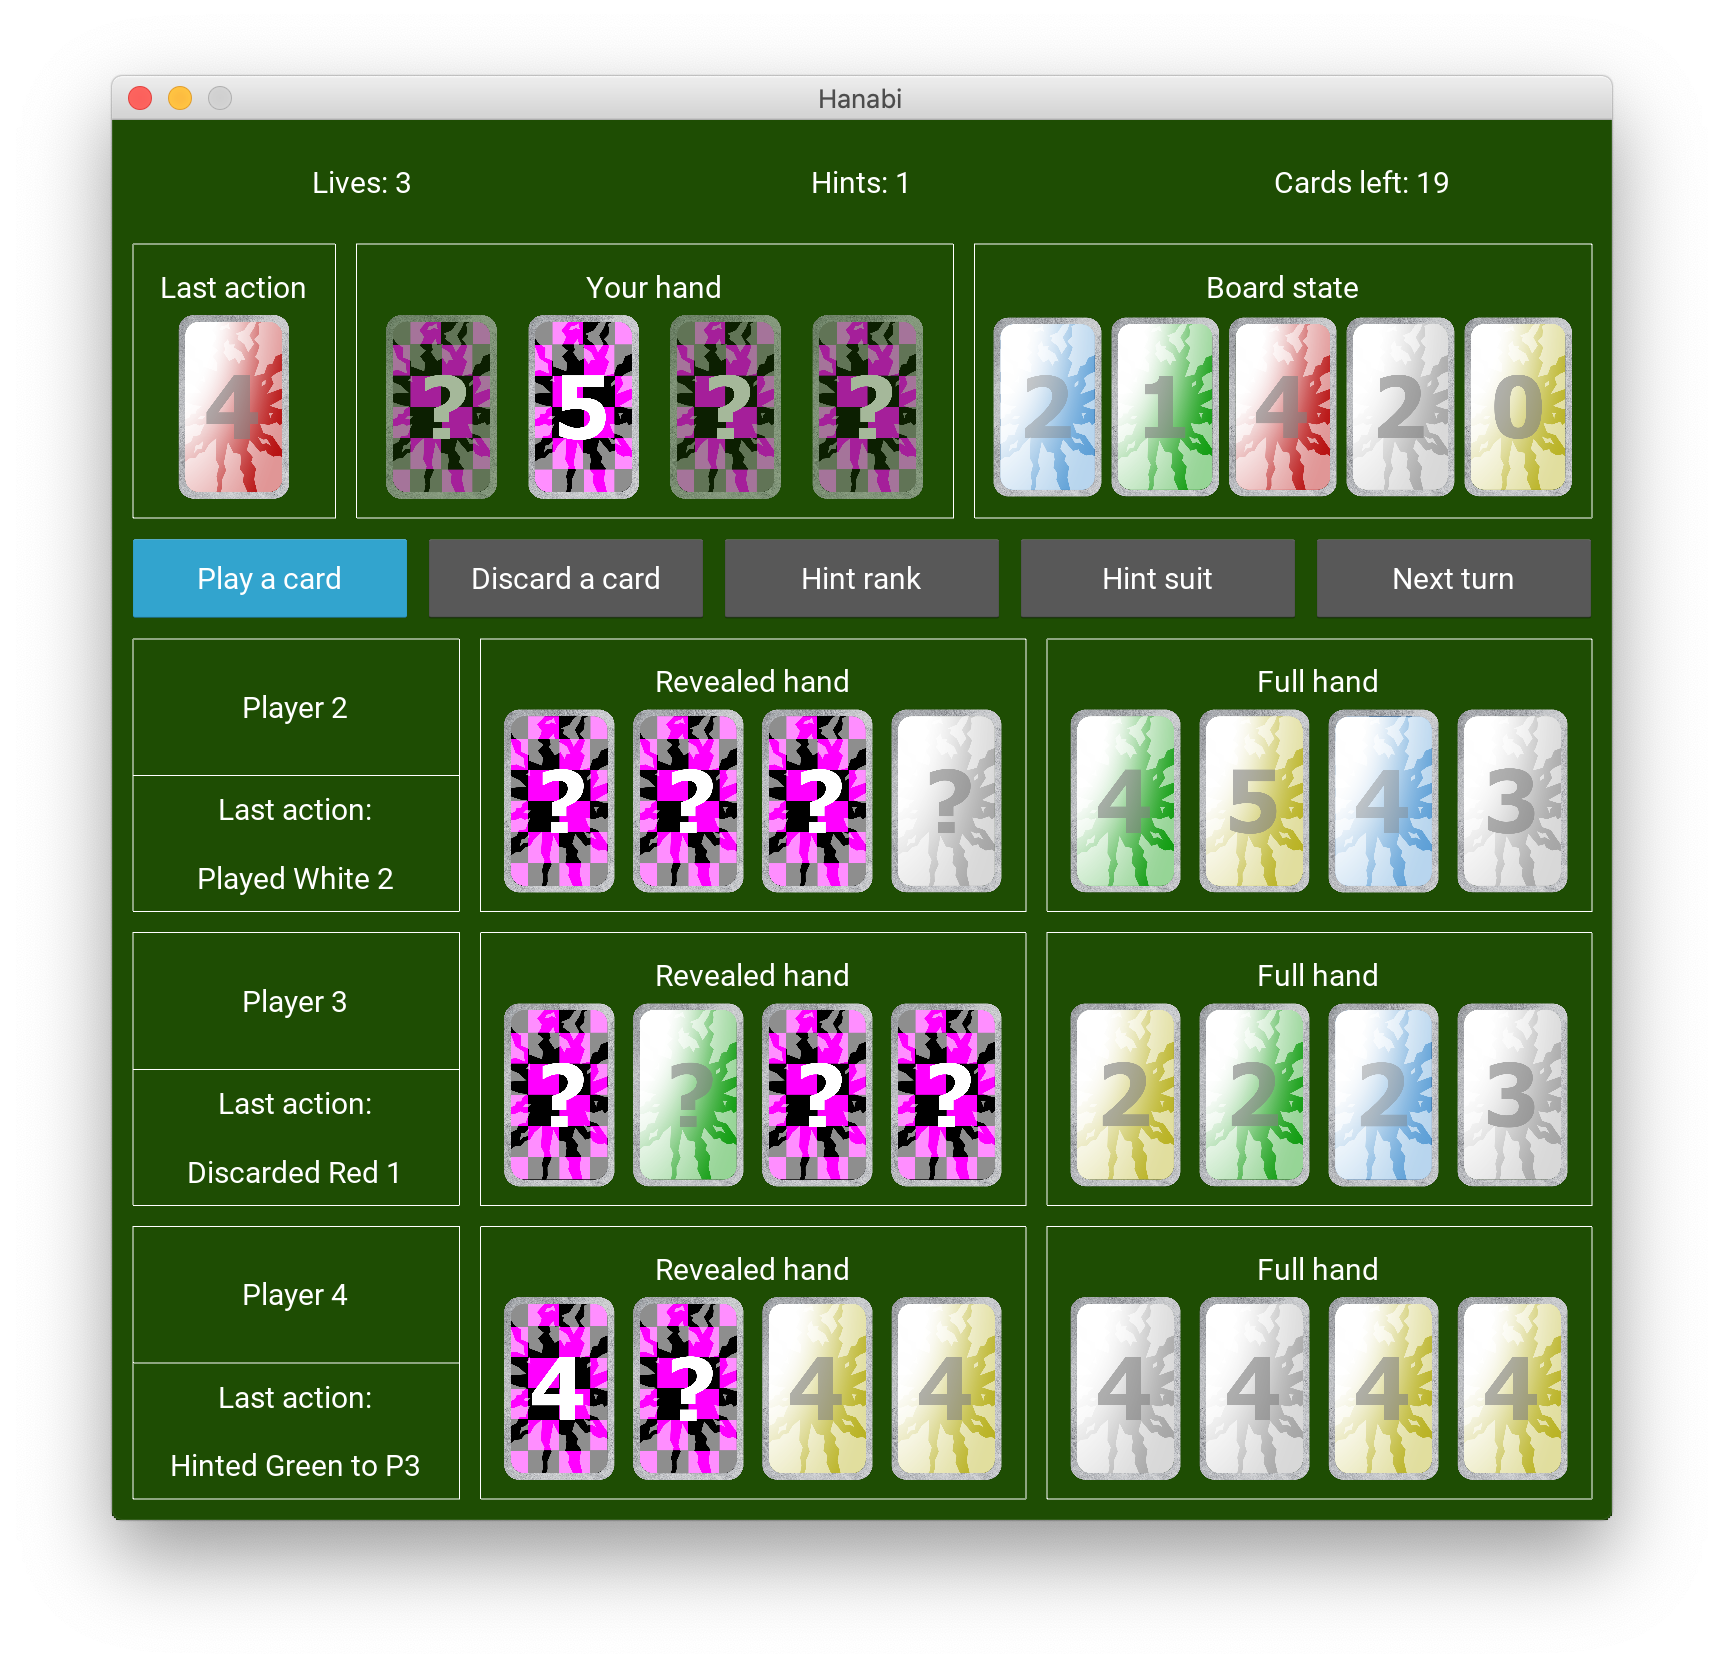
\includegraphics[width=1.0\linewidth]{gui.png}
	\caption[Caption]{Interfejs graficzny do gry Hanabi, utworzony na potrzeby projektu (twórca grafik: Jakub Podwysocki)}
\end{figure}

\section{Wyjaśnienie zasad}

Celem gry jest zdobycie możliwie największej ilości punktów poprzez poprawne zagrywanie kart. Maksymalna ilość możliwych do~uzyskania punktów wynosi dwadzieścia pięć. Po~zakończeniu gry ilość uzyskanych punktów oblicza~się poprzez zsumowanie wartości najwyższych kart z~każdego ze~stosów odpowiedniego koloru.

Talia do~gry składa~się z~pięćdziesięciu kart. Każda karta jest~oznaczona jednym z~pięciu kolorów (czerwony, żółty, niebieski, biały, zielony) oraz jedną z~wartości z~zakresu od~1~do~5. Dla każdego koloru istnieją po~trzy karty o~numerze~1, po~dwie karty o~numerach 2,~3~i~4, a~także po~jednej karcie o~numerze~5.

Na początku gry talia jest tasowana. Gracze rozpoczynają rozgrywkę z~ośmioma żetonami podpowiedzi i~trzema żetonami życia. Żetony te są wspólne dla wszystkich uczestników rozgrywki. Jeżeli graczy jest dwóch lub~trzech, każdy z~nich dobiera po~pięć zakrytych kart. Jeżeli jest ich~czterech lub~pięciu, dobierają po~cztery zakryte karty. Następnie gracze po kolei wykonują swoje ruchy. Ruchu nie~można pominąć. Ruch to~wykonanie jednej z~trzech dostępnych akcji:
\begin{enumerate}
	\item Zagranie karty:

	Gracz deklaruje chęć zagrania karty, wybiera zakrytą ze~swojej ręki, a~następnie wykłada ją~na~stół w~pozycji odkrytej. Zagranie może być~poprawne lub~niepoprawne. Karty muszą być~zagrywane w~kolejności rosnącej, zaczynając od~jedynki, inaczej zagranie uważa~się za~niepoprawne. Przykładowo, jeśli na~stole~nie ma~żadnych kart, można poprawnie zagrać tylko te, które są oznaczone numerem~1. Jeżeli na~stole znajdują~się wyłącznie jedna niebieska karta o~numerze~1 i~stos żółtych kart, spośród których największą wartość ma~karta o~numerze~4, można poprawnie zagrać niebieską kartę o~numerze~2, żółtą kartę o~numerze~5 lub dowolną kartę innego koloru o~numerze~1. Jeżeli karta została zagrana poprawnie, jest ona dodawana do~stosu o~odpowiednim kolorze lub~też~rozpoczyna stos swojego koloru, jeżeli jest to~karta o~numerze~1. Dodatkowo, jeżeli zagrana karta ma~numer~5, gracze otrzymują jeden żeton podpowiedzi (chyba, że~mają ich już osiem -~wtedy zagranie nie~ma~żadnego dodatkowego efektu). Jeżeli karta została zagrana niepoprawnie, jest ona~usuwana z~gry i~nie~jest dodawana do~żadnego ze~stosów, a~gracze tracą jeden z~żetonów życia. Po~rozpatrzeniu efektów akcji gracz dobiera zakrytą kartę z~talii (jeżeli nie~jest ona~pusta).
	
	\item Odrzucenie karty:
 
	Gracz deklaruje chęć odrzucenia karty, wybiera zakrytą ze~swojej ręki, a~następnie wykłada ją~na~stół w~pozycji odkrytej. Karta ta~jest usuwana z~gry, bez dokładania jej~do~któregokolwiek ze~stosów, a~gracze otrzymują jeden żeton podpowiedzi (chyba, że~mają ich już osiem -~wtedy odrzucenie karty nie~ma~żadnego dodatkowego efektu). Po~rozpatrzeniu efektów akcji gracz dobiera zakrytą kartę z~talii (jeżeli nie~jest ona~pusta).

	\item Udzielenie podpowiedzi innemu graczowi:

	Gracz usuwa jeden z~żetonów podpowiedzi, po~czym wybiera innego uczestnika rozgrywki oraz jeden z~dwóch rodzajów informacji, których chce mu~udzielić: może wskazać wszystkie jego karty o~wybranym kolorze lub~wszystkie jego karty o~wybranym numerze. Akcji tej nie~można wykonać, jeśli w~grze~nie ma~żadnych żetonów podpowiedzi, gdyż wiązałoby~się to~z~koniecznością usunięcia żetonu podpowiedzi, który~nie istnieje. Udzielanie graczom podpowiedzi dotyczących kart w~jakikolwiek inny sposób jest zabronione.
\end{enumerate}

Jeżeli któryś z graczy dobierze ostatnią kartę z~talii, każdy uczestnik rozgrywa jedną dodatkową turę (wraz z~graczem, który dobrał ostatnią kartę), po~czym gra~się kończy.

Gra natychmiast kończy~się, gdy~zostanie utracony ostatni żeton życia lub gdy~wszystkie stosy odpowiednich kolorów zostaną skompletowane (czyli na~każdy z~nich poprawnie położono kartę o~numerze~5).

\section{Dodatkowe obserwacje}

Z powodu losowej natury gry, niektórych rozdań nie~da~się wygrać z~maksymalną ilością punktów. Najprostsza taka sytuacja ma~miejsce, gdy w~rozgrywce na~dwóch graczy jeden z~nich dobierze same karty o~numerze~5, drugi dobierze wyłącznie karty o~numerze~4, a~na~górze talii znajdują~się pozostałe karty o~numerze~4. Aby uzyskać dostęp do~kart o~innych numerach, gracze muszą odrzucić (lub niepoprawnie zagrać) co~najmniej sześć kart. Z~zasady szufladkowej można wywnioskować, że~wszystkie kopie co~najmniej jednej z~kart danego rodzaju zostaną bezpowrotnie usunięte z~gry bez umieszczania ich na~stosie, co~uniemożliwia wygraną.

Ze~względu na~ograniczony rozmiar talii, zagrywanie wyłącznie tych kart, o~których posiada~się komplet informacji, jest wysoce nieefektywne. Po~rozdaniu kart graczom talia zawiera~od~30~do~40 kart, zależnie od~liczby graczy. Aby uzyskać najwyższy wynik, należy zagrać aż~25~kart, a~zagranie każdej z~nich oznacza zmniejszenie rozmiaru talii o~jeden. Oznacza to (zakładając, że~gracze próbują uzyskać 25~punktów), że~można wykonać maksymalnie od~10~do~17 ruchów, w~których odrzuca~się kartę, wliczając w~to~tury po~opróżnieniu talii. Po~doliczeniu początkowych 8~żetonów daje to~maksymalną ilość 25~podpowiedzi. Oznacza to, że~w~grze na~dwie osoby każda podpowiedź musi jednoznacznie ujawniać średnio po~jednej karcie, lecz każda z~nich potrzebuje dwóch podpowiedzi różnego rodzaju, by~uzyskać pełną informację. Przy pięciu graczach każda podpowiedź musi średnio ujawniać już nie~jedną, a~prawie półtorej karty.

Ponadto, jeżeli chcemy odrzucać wyłącznie karty, które można bezpiecznie usunąć z~gry, inni gracze muszą nam zakomunikować ich brak przydatności poprzez odpowiednie podpowiedzi (lub ich brak, co~jest w znacznym stopniu utrudnione przez konieczność udzielania pełnej informacji o~zawartości ręki współuczestników). Karty bezużyteczne mogą, lecz nie~muszą zostać ujawnione w~drodze przypadku, podczas ujawniania innych kart. W~rezultacie najczęściej przyjmowaną konwencją wśród graczy jest odrzucanie najstarszej karty w~ręce: jeżeli żaden z~uczestników rozgrywki nie~ostrzega przed usunięciem jej z~gry, istnieje wysokie prawdopodobieństwo, że~jest ona nieprzydatna.

\chapter{Strategie sztucznej inteligencji}

\section{Podejście regułowe}

Podczas realnej rogrywki Hanabi gracze nie dysponują komputerem, który pomagałby im~w~wykonywaniu ruchów poprzez dokonywanie odpowiednich obliczeń. Zamiast tego korzystają oni z~wiedzy nabytej w~trakcie rozegranych już partii, modyfikując swoje strategie i~rozszerzając je~o~kolejne elementy, aż~do~osiągnięcia zadowalającego ich poziomu wiedzy o~grze. Proces ten w~naturalny sposób prowadzi do~wykształcenia konwencji (takich jak: ``należy zawsze odrzucać najstarszą kartę na~ręce''), a~także do~opracowania systemu reguł, pomocnych w~uzyskiwaniu wysokich wyników (przykładowo: ``jeżeli ktoś chce odrzucić ważną kartę, należy go~powstrzymać poprzez udzielenie odpowiedniej podpowiedzi''). Zasady te~można przełożyć na~algorytmy, co~prowadzi do~utworzenia systemów regułowych, znanych także jako eksperckie.

Algorytmy regułowe to~programy, które poprzez procesy decyzyjne naśladują wybory, których w~danych sytuacjach mógłby dokonać człowiek. Są~one najczęściej deterministyczne, co~jest cechą szczególnie ważną w~środowiskach, które wymagają koordynacji i~przewidywania działań podejmowanych przez inne elementy systemu. W~przypadku agentów sztucznej inteligencji, algorytmy regułowe powielają zachowania prawdziwych graczy.

Z~racji na kooperacyjną konstrukcję Hanabi, sama emulacja typowych zachowań ludzkich graczy~nie wystarcza jednak, by~wygrać. Potrzebna jest także odpowiednia koordynacja działań pomiędzy agentami: strategia. Gracze muszą zwracać uwagę na~współuczestników rozgrywki i~na~bieżąco interpretować ich poczynania, by~móc wywnioskować, jaka seria ruchów doprowadzi do~najlepszej możliwej sytuacji. Prostym i~efektywnym sposobem na~zaimplementowanie strategii jest wyspecyfikowanie protokołu komunikacji pomiędzy agentami, który nadaje niektórym zagraniom dodatkowe znaczenie, rozumiane przez pozostałych graczy. Przykładowo, dobrym pomysłem może być zasada o~następującej treści: ``jeżeli inny gracz podpowiedział mi bez wyraźnej przyczyny jeden z kolorów, ujawniając w ten sposób kilka kart, najprawdopodobniej mogę je zagrać, w~kolejności od~lewej do~prawej''. Z~tego powodu implementacja agentów regułowych wiąże~się z~koniecznością bardzo dobrej znajomości zasad rządzących grą.

\section{Drzewa poszukiwań}

Istnieją dwa główne czynniki, które sprawiają, że~analiza stanu gry w~Hanabi jest trudnym zadaniem. Są~to: niepełna informacja o~aktualnym etapie rozgrywki, a~także losowość kart dobieranych z~talii. Udowodniono, że~nawet w uproszczonej wersji gry, w~której uczestnicy mogą patrzeć na~swoje karty, problem perfekcyjnego zagrania jest NP-kompletny\cite{NP-Complete}. Sprawia to, że~podejście do~zagadnienia w~sposób siłowy jest nieefektywne. Fakt ten, połączony z~trudnością opracowania funkcji oceniającej jakość zagrania, wyklucza użycie części możliwych rozwiązań problemu, takich jak algorytm alfa-beta.

Aby obejść trudność znalezienia perfekcyjnego zagrania, grupa Facebook Research zaproponowała rozwiązanie bazujące na~drzewie poszukiwań Monte Carlo\cite{MCTS}. Każdy z~graczy dysponuje zbiorem predefiniowanych akcji, które dostosowuje odpowiednio do~aktualnego stanu rozgrywki poprzez analizę prawdopodobieństwa zagrań, które mogą wykonać współuczestnicy. Algorytm bierze pod uwagę także szanse aktualnego gracza na~posiadanie w~ręce kart, które mogły zostać wylosowane z~talii. Aby przyspieszyć działanie programu, głębokość drzewa poszukiwań jest ograniczana, a agenci wykonują predefiniowane akcje i~nie~eksplorują nowych opcji, jeżeli wiązałoby~się to~z~przekroczeniem zadanego limitu obliczeń. 

Takie podejście pozwala na uzyskanie bardzo wysokich wyników, sięgających nawet 24.61~punktów w~rozgrywce dla dwóch graczy. Działanie algorytmu jest jednak kosztowne obliczeniowo, nawet przy znacznym ograniczeniu zakresu dokonywanych poszukiwań. Do~osiągnięcia tak wysokich punktacji potrzeba olbrzymich ilości obliczeń, które, z racji na możliwość ich zrównoleglenia, są~najczęściej dokonywane na~nowoczesnych kartach graficznych. Wyłączenie agentom możliwości dokonywania dodatkowych poszukiwań degeneruje je~do~agentów regułowych, które, choć na~każdą akcję potrzebują zużycia istotnie mniejszej ilości zasobów, wciąż osiągają imponujący wynik 23~punktów.

\section{Algorytmy uczące}

Innym sposobem na~zaimplementowanie programu grającego w Hanabi jest użycie algorytmów uczących, które łączą zalety podejść regułowych i~poszukujących. Jak sugeruje nazwa, polegają one na~symulowaniu procesu akumulacji doświadczenia, podobnego do~tego doznawanego przez ludzkich graczy. W~toku ewolucji agent zdobywa wiedzę o~środowisku, w~którym operuje, dostosowując~się do~zmieniających warunków, wypracowując i~udoskonalając sposoby radzenia sobie w~zaprezentowanych sytuacjach. Tworzenie algorytmów uczących nie~wymaga ani szerokiej wiedzy o~zawiłościach zasad gry, ani kosztownych obliczeń, które byłyby wykonywane w~trakcie rozgrywki.

Wadą tego podejścia jest konieczność wyuczenia agenta odpowiednich zachowań. Odbywa~się to~poprzez zapewnienie mu~zestawu danych, na~których mógłby zdobyć doświadczenie. W~zależności od~uzyskiwanych wyników, decyzje algorytmu są~nagradzane lub karane. Dobranie odpowiednio różnorodnego zbioru uczącego, w~parze z funkcjami kwalifikującymi, pozwala programowi nie~tylko na~rozpoznawanie i~radzenie sobie z~najczęściej występującymi sytuacjami, ale i~generalizację zachowań, potrzebną do~wybrnięcia ze~stanów gry, które nie~zostały dotychczas napotkane.

Należy mieć na~uwadze, że~nieodpowiedni dobór zbioru uczącego lub funkcji, które oceniają poczynania agenta, potrafią doprowadzić do~anomalii w~procesie zdobywania wiedzy. Jeżeli zestawy testowe będą zbyt homogeniczne i~liczne w~stosunku do~osiągalnej liczby stanów rozgrywki, może dojść do~przeuczenia modelu, z~kolei zbyt krótka nauka nie~przygotowuje programu do~nietypowych sytuacji. Nieprawidłowości w~procedurach klasyfikujących, choć mniej zauważalne, także potrafią doprowadzić do~niepożądanych sytuacji, tak jak miało to~miejsce w~przypadku programu grającego w~produkcje na~platformę Nintendo Entertainment System. Agent ten, nie~chcąc doprowadzić do~przegranej, nauczył~się wstrzymywać rozgrywkę na~zawsze\cite{Mario}.

\section{Naginanie zasad gry}

W~oficjalnych zasadach gry nie~ma~wyszczególnionego przymusu udzielania podpowiedzi, które ujawniałyby jakiekolwiek karty. Jeżeli wybierzemy gracza, który~nie posiada żadnych czerwonych kart i~zdecydujemy się na~podpowiedzenie mu~czerwonego koloru, tura jest pomijana za~cenę żetonu podpowiedzi. Choć taki ruch wydaje~się~nie mieć sensu, gdyż podpowiedź można wykorzystać w~produktywny sposób, otwiera on~możliwość poważnego nagięcia zasad gry. Jeżeli każdej z~możliwych podpowiedzi przypiszemy unikatową wartość numeryczną, możemy za~ich pomocą przekazywać innym graczom informacje liczbowe. Jest to~powód, dla~którego możliwość udzielania pustych podpowiedzi jest uznawana w~społeczności graczy Hanabi za~kontrowersyjną, toteż w~niektórych edycjach gry została ona zakazana.

Fakt ten można wykorzystać do~stworzenia agenta, który za~pomocą pozornie bezwartościowych ruchów udziela podpowiedzi wszystkim graczom jednocześnie. Korzysta on~ze~słynnej zagadki logicznej, znanej jako problem więźniów i~kapeluszy, odpowiednio uogólnionej i~dopasowanej do~liczby graczy. Agent, który rozgrywa aktualną turę, oblicza idealne zagrania dla~innych uczestników rozgrywki, po~czym szyfruje je~do~postaci liczbowej. Kolejni gracze, znając podaną przez poprzednika wartość, po~rozpatrzeniu optymalnych zagrań innych graczy, są~w~stanie wywnioskować, jaki ruch powinni wykonać.

Według badań z 2017 roku\cite{HatPlayer}, agent ten uzyskuje maksymalną ilość punktów średnio w~92\%~rozgrywanych gier, co jest wynikiem bliskim optymalnemu. Jest to~imponujący rezultat, zarówno ze~względu na~bardzo szybkie działanie algorytmu, jak i~jego nadzwyczajną efektywność.

Niestety, taki sposób gry całkowicie zawodzi, gdy jeden z~graczy wyłamie się z~konwencji narzuconej przez protokół komunikacji. Dodatkowo, algorytm działa wyłącznie w~rozgrywce na~czterech oraz pięciu graczy, gdyż głównym powodem jego sukcesu jest możliwość przekazywania w~każdej z~podpowiedzi maksymalnej ilości informacji, a~zmniejszenie ilości graczy powoduje znaczne zredukowanie efektywności ruchów. Są~to~powody, dla których agent ten nie~nadaje~się do~rozgrywki z~człowiekiem.

\chapter{Ujęcie praktyczne}

WIP

\chapter{Wyniki eksperymentów}

WIP

\begin{thebibliography}{3}

\bibitem{NP-Complete} J.-F Baffier i in., \textit{Hanabi is NP-complete, Even for Cheaters who Look at Their Cards}, 2017. URL: 
\href{https://arxiv.org/pdf/1603.01911.pdf}{\textbf{link}} (term. wiz. 11.01.2020)

\bibitem{MCTS} A. Lerer, H. Hu, J. Foerster, N. Brown, \textit{Building AI that can master complex cooperative games with hidden information}, 2019. URL: 
\href{https://ai.facebook.com/blog/building-ai-that-can-master-complex-cooperative-games-with-hidden-information/}{\textbf{link}} (term. wiz. 11.01.2020)

\bibitem{Mario} B. Bouzy, \textit{The First Level of Super Mario Bros. is Easy with Lexicographic Orderings and Time Travel . . . after that it gets a little tricky.}, 2013. URL: 
\href{http://www.cs.cmu.edu/~tom7/mario/mario.pdf}{\textbf{link}} (term. wiz. 11.01.2020)

\bibitem{HatPlayer} B. Bouzy, \textit{Playing Hanabi Near-Optimally}, 2017. URL: 
\href{http://helios.mi.parisdescartes.fr/~bouzy/publications/bouzy-hanabi-2017.pdf}{\textbf{link}} (term. wiz. 11.01.2020)

\end{thebibliography}

\end{document}
